\documentclass[12pt]{exam}
\usepackage[utf8]{inputenc}		% Caracteres latinos
\usepackage[spanish]{babel}		% Idioma español
\usepackage{geometry}			% Organizar el documento
\usepackage{graphicx}			% Incluir gráficos
\usepackage{makecell}			% Para personalizar las celdas de una tabla
\usepackage[nohdr]{mathexam}	% Añadimos el paquete mathexam (sin header)
\usepackage{amsmath}
\usepackage{amsfonts}
\usepackage{amssymb}
\usepackage{mathtools}
\usepackage{tikz,pgfplots}
\usepgfplotslibrary{polar}
\usepackage[shortlabels]{enumitem}
 \renewcommand{\baselinestretch}{1.5}
\usepackage{mathtools}
\usepackage{bm}
\usepackage{esvect}
\usepackage[fleqn]{mathtools}
\usepackage{relsize}
\usepackage{multirow}
\usepackage{multicol}
\usepackage[document]{ragged2e}
 \usepackage{textpos}
\usepackage{tcolorbox}
\usepackage{hyperref}
\usepackage{mathdesign}

%\usepackage[]{mathptmx}        % A free version o Times Roman with mathematical symbols
%\usepackage{pzc}               % fuente cursiva (conjuntos) Zapf Chancery
%\usepackage{showframe}
%\usepackage{lipsum}

% DOCUMENTACIÓN DE LA CLASE EXAM
% http://ftp.inf.utfsm.cl/pub/tex-archive/macros/latex/contrib/exam/examdoc.pdf
% DOCUMENTACIÓN DE LA CLASE MATHEXAM
% http://ctan.dcc.uchile.cl/macros/latex/contrib/mathexam/doc/mathexam.pdf

% Definimos la geometría de la primera página
\geometry{
	a4paper,                    % Tamaño del documento
	hmargin = {1.7cm, 1.6cm}, 	% Margen horizontal izquierdo, derecho
	vmargin = {1cm, 1cm},	    % Margen vertical superior, inferior
	headsep = 4mm,				% Separación entre el encabezado y el texto
	head = .2cm,				% Tamaño del encabezado
	% marginparsep = 5mm, 		% Seperación entre las notas y el texto
	% marginpar = 1.5cm,		% Tamaño de las notas
	includeall,                 % incluye el encabezado, footer y notas dentro del tamaño del documento
	nomarginpar,	            % Elimina las notas
	foot = 1cm,                 % Tamaño del footer
	twoside,                	% Habilita el modo de impresión a doble cara
}

\selectlanguage{spanish}        % Selecciona el idioma
\spanishdecimal{.}

%\pagestyle{headandfoot}         % Nuestro examen tendrá encabezado y pié

% DEFINIMOS EL ENCABEZADO
%\header{
%\begin{tabular}{l c c c l}
%            \makecell{\includegraphics[height=2.5cm]{logo.png}} &
%            \makecell{\textbf{IPEA 215} \\Raúl Scalabrini Ortiz} &
%            \makecell{Examen} &
%            \makecell{Curso\\1er Año} &
%             \makecell[l]{Apellido y %Nombre:\enspace\makebox[2in]{\hrulefill}\\Fecha: \today}
%        \end{tabular}}{}{}

% DEFINIMOS EL PIE
%\rfoot{Página \thepage\ de \numpages}
\newcommand{\iuni}{\pmb{\hat{\imath}}}
\newcommand{\juni}{\pmb{\hat{\jmath}}}
\newcommand{\kuni}{\pmb{\hat{k}}}
\renewcommand{\sin}{\,\text{sen}\,}

% DOCUMENTO
\begin{document}

\centering


\Large 
\textbf{\huge Tarea 6 \\ \large Generalidades de sistemas de ecuaciones}

\small
Fecha de entrega lunes 13 de Diciembre
\vskip10pt
% \flushleft
% \begin{tcolorbox}
% LEE ANTES DE COMENZAR LA TAREA
% \begin{enumerate}
%     \item Se califica sobre 10 por lo que es posible obtener 13 si se realizan también los ejercicios opcionales.
%     \item El ejercicio opcional puede sustituir a uno y solo uno de los ejercicio del bloque previo.
%     \item Subir el archivo en \textbf{PDF} a la plataforma con las páginas numeradas.

% \end{enumerate}
% \end{tcolorbox}
\normalsize

\pointpoints{punto}{puntos}
\pointformat{\bfseries\boldmath(\thepoints)}
\vskip10pt

    
    \begin{questions}
     % 1 % 
     \question% Blanchard S2.1 e1-6 
     Los incisos a - f se refieren a los siguientes sistemas de ecuaciones:
     
     $
     \begin{array}{lrclclrcl}
        i)&\frac{dx}{dt}& = & 10x\left(1-\frac{x}{10}\right)-20xy& &ii)& \frac{dx}{dt} & = & 0.3x-\left(\frac{xy}{100}\right)\\
        & \frac{dy}{dt} & = & -5y+\frac{xy}{20} & & &\frac{dy}{dt}& = & 15y\left(1-\frac{y}{15}\right)+25xy
     \end{array}
     $
     \begin{enumerate}[a)]
         \item En uno de esos sistemas, las presas son animales muy grandes y los depredadores son animales muy pequeños, tales como elefantes y mosquitos. Se requieren entonces muchos de éstos para cazar una presa, pero cada animal devorado proporciona gran beneficio para la población depredadora. El otro sistema tiene depredadores muy grandes y presas muy pequeñas. Identifica cada sistema y da una justificación para tu respuesta.
         \item Encuentra todos los puntos de equilibrio para los dos sistemas. Explica la importancia de esos puntos en términos de las poblaciones presa y depredadora.
         \item Supón que los depredadores están extintos en el tiempo $t_0=0$. Para cada sistema, comprueba que éstos permanecen extintos en todo tiempo.
         \item Para cada sistema, describe el comportamiento de la población presa si los depredadores están extintos. Suponiendo que no hay depredadores, esboza la línea fase y también las gráficas para la población presa como función del tiempo para varias soluciones. Después interprétalas para esta misma población.
         \item Para cada sistema, supón que las presas están extintas en el tiempo  $t_0=0$. Verifica que la extinción perdura para todo tiempo.
         \item Para cada sistema, describe el comportamiento de la población depredadora si las presas están extintas. Tomando en cuenta la ausencia de presas, bosqueja la línea fase y las gráficas de la población depredadora como función del tiempo para varias soluciones. Interpreta luego esas gráficas para la población depredadora.
     \end{enumerate}


     % 2 % Blanchard S2.2 e17-20 Paul S2.2 11
     \question% 
     Determina el sistema que corresponda a cada uno de los campos direccionales y justifica tu respuesta.
     \begin{enumerate}[I)]
         \item $\frac{dx}{dt}=-x\atop \frac{dy}{dt}=y-1$\vskip7pt
         \item $\frac{dx}{dt}=x\atop \frac{dy}{dt}=2y$\vskip7pt
         \item $\frac{dx}{dt}=x^2-1\atop \frac{dy}{dt}=y$\vskip7pt
         \item $\frac{dx}{dt}=x-1\atop \frac{dy}{dt}=-y$\vskip7pt
         \item $\frac{dx}{dt}=x+2y\atop \frac{dy}{dt}=-y$\vskip7pt
         \item $\frac{dx}{dt}=x^2-1\atop \frac{dy}{dt}=-y$\vskip7pt
         \item $\frac{dx}{dt}=2x\atop \frac{dy}{dt}=y$
         \item $\frac{dx}{dt}=x-2y\atop \frac{dy}{dt}=-y$
     \end{enumerate}
     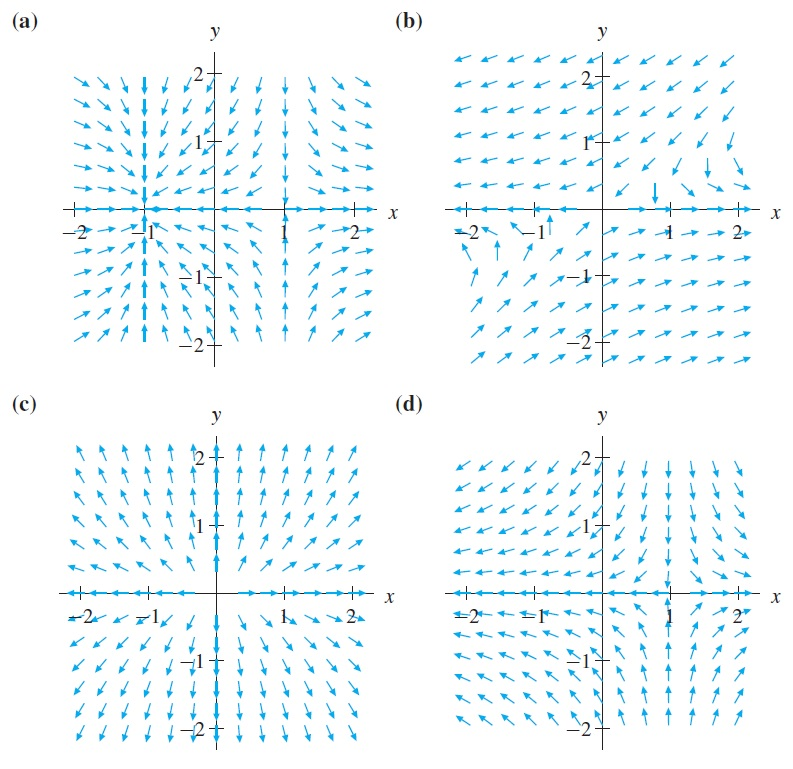
\includegraphics[scale=.7]{F1T6.jpg}

     
     % 3 % Blanchard S2.2 e7 Paul S2.2 e8
     \question% 
     Convierte la ecuación diferencial de segundo orden $$\frac{d^2y}{dt^2}-y=0$$ en un sistema de primer orden en términos de $y$ y $v$, donde $v=dy/dt$, y
     \begin{enumerate}[a)]
         \item determina el campo vectorial asociado con el sistema de primer orden,
        %  \item dibuja suficientes vectores en el campo vectorial para tener una idea de su estructura geométrica,
         \item esboza el campo de direcciones asociado, y 
         \item realiza un croquis del retrato fase del sistema.
     \end{enumerate}


     % 4 % Blanchard  S2.3 e19a,b,c
     \question% 
     Considera el sistema parcialmente acoplado $$\begin{array}{rcl}
          \frac{dx}{dt}&=&xy  \\
          \frac{dy}{dt}&=&y+1 
     \end{array}$$
     \begin{enumerate}[a)]
         \item Obtén la solución general.
         \item Calcula los puntos de equilibrio del sistema.
         \item Encuentra la solución que satisface la condición inicial $(x_0,y_0)=(1,0)$.
        %  \item Grafica el retrato fase para este sistema e identifica la curva solución que corresponde a la solución con condición inicial $(x_0,y_0)=(1,0)$. (Apóyate en una calculadora o computadora)
     \end{enumerate}


     % 5 % Blanchard  S2.3 e1-4
     \question%
     Considera el sistema $$\begin{array}{rcl}
          \frac{dx}{dt}&=&2x+2y  \\
          \frac{dy}{dt}&=&x+3y 
     \end{array}$$
     Para las funciones dadas $\mathbf{Y}(t)=(x(t),y(t))$, comprueba si $\mathbf{Y}(t)$ es solución del sistema:
     \begin{enumerate}[a)]
         \item $(x(t),y(t))=(2e^t,-e^t)$
         \item $(x(t),y(t))=(3e^{2t}+e^t,-e^t+e^{4t})$
        %  \item $(x(t),y(t))=(2e^t-e^{4t},-e^t+e^{4t})$
        %  \item $(x(t),y(t))=(4e^t+e^{4t},-2e^t+e^{4t})$
     \end{enumerate}



     % 6 % Blanchard S2.4 e2
     \question% 
     Para el sistema $$\frac{dx}{dt}=2x\atop \frac{dy}{dt}=y$$
     afirmamos que la curva $\mathbf{Y}(t)=(e^{2t},3e^t)$ es una solución. Su posición inicial es $\mathbf{Y}(0)=(1,3)$.
     \begin{enumerate}[a)]
         \item Verifica que $\mathbf{Y}(t)=(e^{2t},3e^t)$ es una solución.
         \item Usa el método de Euler con tamaño de paso $\Delta t=0.5$ para aproximar esta solución y determina su cercanía a la solución real cuando $t=2$, $t=4$ y $t=6$.
         \item Ahora usa el método de Euler con tamaño de paso $\Delta t=0.1$ para hacer la aproximación. Calcula que tan cerca está de la solución real cuando $t=2$, $t=4$ y $t=6$.
        %  \item Explica por qué y cómo difieren las aproximaciones de Euler de la solución real.
     \end{enumerate}
     Apóyate en una calculadora o computadora para realizar los cálculos y gráficas. No olvides poner tu codigo.


    %  % 7 % Blanchard S2.4 e5
    %  \question%
    %  Cerca del origen, dondes $x$, $y$ y $z$ son muy pequeñas, los términos combinados $-xz+xy$ serán en extremo pequeños. Entonces, cerca de $(x,y,z)=(0,0,0)$ podemos aproximar el sistema de Lorenz con $$\begin{array}{rcl}
    %       \frac{dx}{dt}&=&10(y-x)  \\
    %       \frac{dy}{dt}&=&28x-y \\
    %       \frac{dz}{dt}&=&-\frac{8}{3}z
    %  \end{array}$$
    %  Observa que $z$ no aparece en las ecuaciones para $dx/dt$ y $dy/dt$ y que la ecuación $dz/dt$ no contiene $x$ o $y$; es decir, el sistema se desacopla en uno dimensional y en una ecuación dimensional.
    %  \begin{enumerate}[a)]
    %      \item Taza el campo de direcciones y el plano fase para el sistema plano $$\frac{dx}{dt}=10(y-x)\atop \frac{dy}{dt}=28x-y$$
    %      \item Esboza la línea fase para la ecuación
    %      $$\frac{dz}{dt}&=&-\frac{8}{3}z$$
    %      \item Bosqueja las soluciones en el espacio de fase tridimensional para el sistema anterior.
    %  \end{enumerate}
    %  \paragraph{Observación:} Esta imagen da el comportamiento del sistema de Lorenz \textit{cerca} de $(0,0,0)$.


     
     
    %  % 8 % 
    %  \question%


     
    %  % 9 % 
    % \question% 


    %  % 10 % 
    %  \question%
     
     
     
    
    %  % 11 %
    %  \question% 
     

    %  % 12 %
    %  \question% 
     
     
        \end{questions}
%         \vskip30pt
%   \RaggedRight
% 	2 PUNTOS EXTRAS %Nagle S4.7 e7,8
	
  

    
    


 
 

 
    
%     \newpage



% Geometría para la otra carilla
\newgeometry{
	hmargin = {1.5cm, 1.5cm},
	vmargin = {5cm, 1cm},
	%nofoot,			% Elimina el pié
	nohead,			% Elimina el encabezado
	nomarginpar,	% Elimina las notas
	includeall,
}% \savegeometry{geometria_1}

\pagestyle{foot}    % El estilo de ésta página sólo constará de pié de página
\runningfooter{}{}{Página \thepage\ de \numpages}


%\lipsum[1-5]

% \restoregeometry
% \loadgeometry{geometria_1}


\end{document}
